\clearpage
\section{LHC and CMS\label{sec:detector}}

The Large Hadron Collider (LHC) is a particle accelerator and collider
housed 100 meters undeground in a 27 km long circualar tunnel situated 
beneath the swiss-french border. The collider consists of two 
counter-circulating particle beams merged and collided at four points 
along the ring. Figure~\ref{fig:lhc} shows the location of the LHC and 
the four main detectors each housed at a different collision point.
The machine also consists of four straight long sections where acceleration, 
collimation, and beam dump systems are held. The longer arc sections are
in fact comprised of 1232 straight dipole magnets 15 meters in length designed to contain 
the particle beams in a circular path. Each sections is held at a 
super-conductive temperature of 2 Kelvin which provides magnetic fields up to 8
Tesla that steer the beams. Higher order multi-pole magnets are 
places near the interaction points to collimate and allign the 
colliding beams. Unwanted beam interaction with residual gas in the beam pipes
is minimized by vacuuming the beam pipes to pressures below $10^{-10}mbar$.

\begin{figure}[h!t]
  \begin{center}
      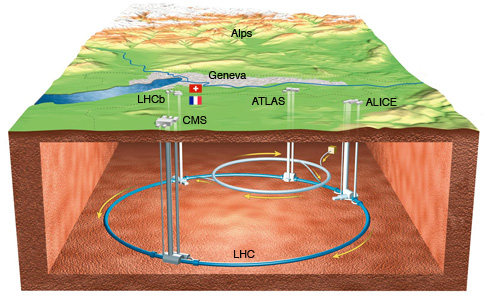
\includegraphics[width=0.40\textwidth,]{figures/CERNMap.jpg}
      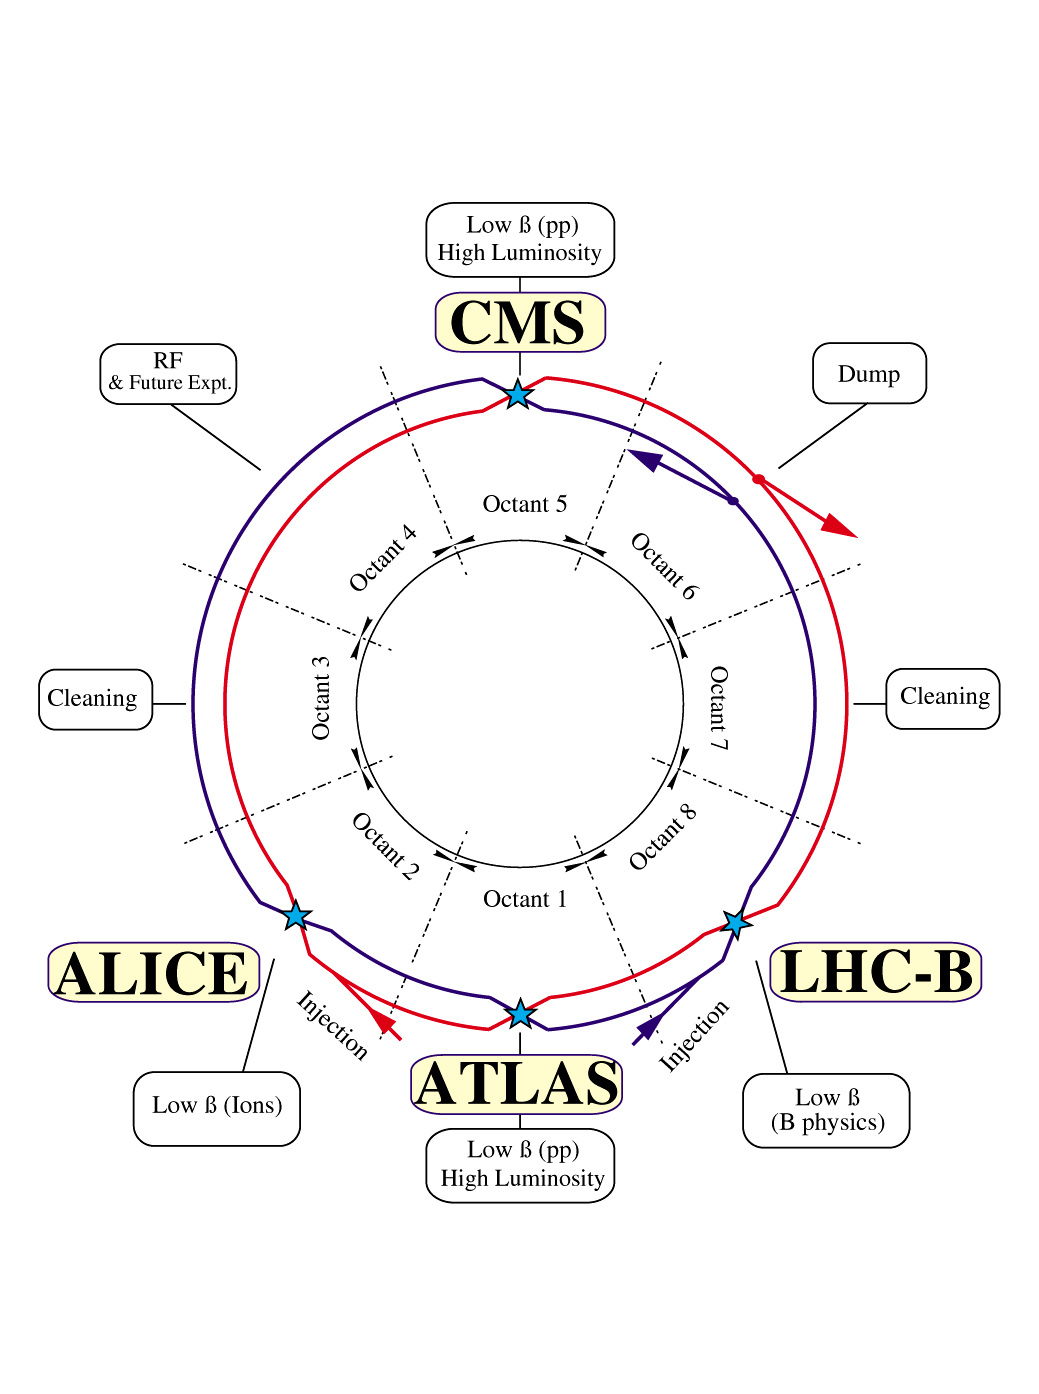
\includegraphics[width=0.35\textwidth,]{figures/lhc-pho-1997-060.jpg}
      \caption{\label{fig:lhc} the lhc}
  \end{center}
\end{figure}

The protons are accelerated along straight sections of the ring where 
Radio-Frequency (RF) cavities generating electromagnetic fields are 
tuned to deliver protons a ‘kick’ of energy at each revolution in the accelerator ring. 
As a result, the energy of the proton allows it to reach velocities close to the speed
of light. Protons that are ideally timed and have exactly the desired energy, will feel 
a zero accelerating force from the RF cavity, while protons with slightly different 
energies that arrive earlier or later are decelerated or accelerated. As a result, 
the proton beams are divided in discrete ‘bunches’ of protons. The LHC has been designed 
to provide 2808 bunches per beam, with about $10^11$ protons per bunch. The figure of merit 
for colliders such as the LHC is the luminosity, a quantity influencing
the rate of collisions. The instantaneous luminosity depends on the number of protons
per beam, the transverse dimensions of the beams (the more the beams are squeezed,
the higher the probability that a proton-proton collision takes place), and the bunch-
crossing frequency. The number of events N of a certain process with cross section σ
produced per second can be expressed as

\begin{equation}
  \label{eq:lumi}
  \frac{dN}{dt} = \,\mathcal{L} \times \sigma
\end{equation}

The luminosity integrated over the course of the three seperate proton-proton collision runs
is shown in figure~\cite{fig:int_lumi}. The large increases in delivered luminosity in such
a short time indicates both the phenomenal success of LHC commissioning and running, and 
the challenge presented to CMS to accommodate new running conditions nearly continuously, 
in particular to design and deploy suitable trigger tables, readout thresholds, 
reconstruction algorithms, and analysis methods.

\begin{figure}[h!t]
  \begin{center}
      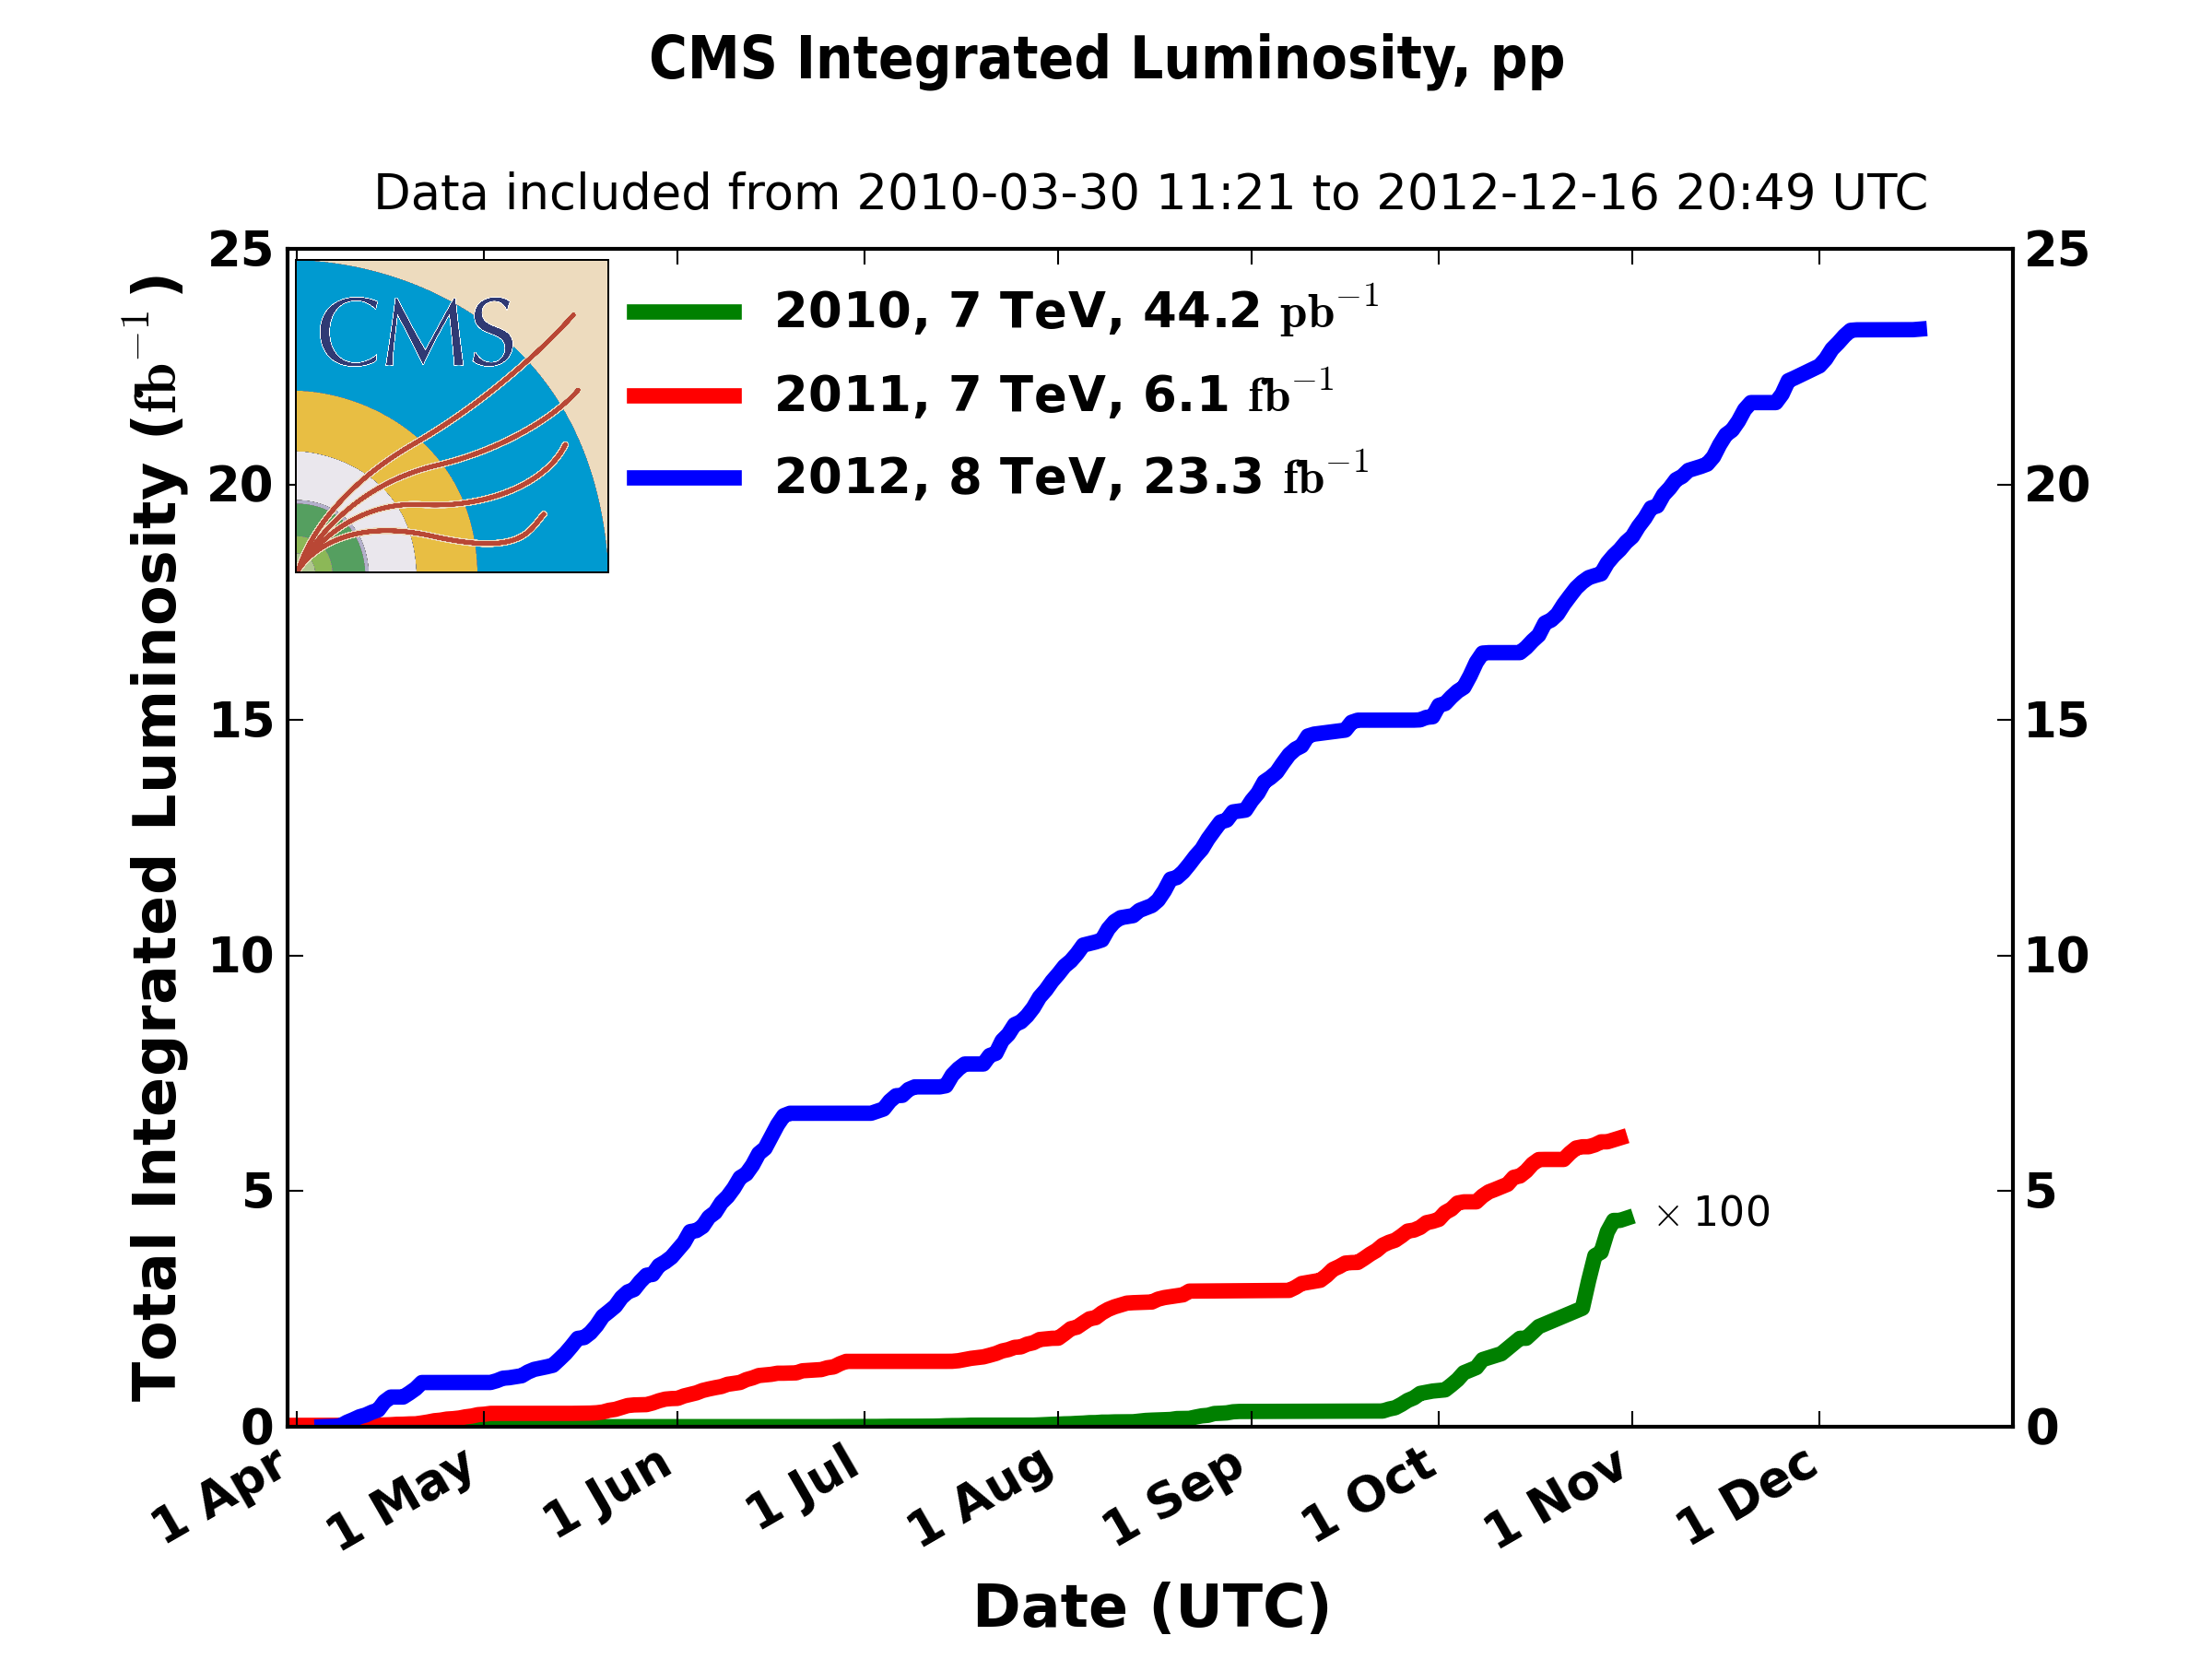
\includegraphics[width=0.40\textwidth,]{figures/int_lumi_cumulative_pp_2.png}
      \caption{\label{fig:int_lumi} the lhc}
  \end{center}
\end{figure}

The interactions sought and the SM processes that appear as backgrounds are those in 
which substantial momentum is transferred between the constituent partons of the LHC’s 
colliding protons; the incident protons are destroyed and energetic outgoing elementary 
particles and proton remnants are produced. The distributions of what fraction of a 
proton’s momentum a constituent gluon or quark carries are given by parton distribution 
functions (PDFs). For a particular production process, e.g. $pp \ra \ttbar$ or 
$pp \ra \bar{g}\bar{g}$, there are various parton scattering processes, e.g. 
from initial gg or $q\bar{q}$, which contribute; their cross sections are integrated over momentum fraction according to 
the PDFs and summed to obtain a total production cross section.
Results of such cross section computations for a variety of processes are shown
in Figure 2.4. 

\begin{figure}[h!t]
  \begin{center}
      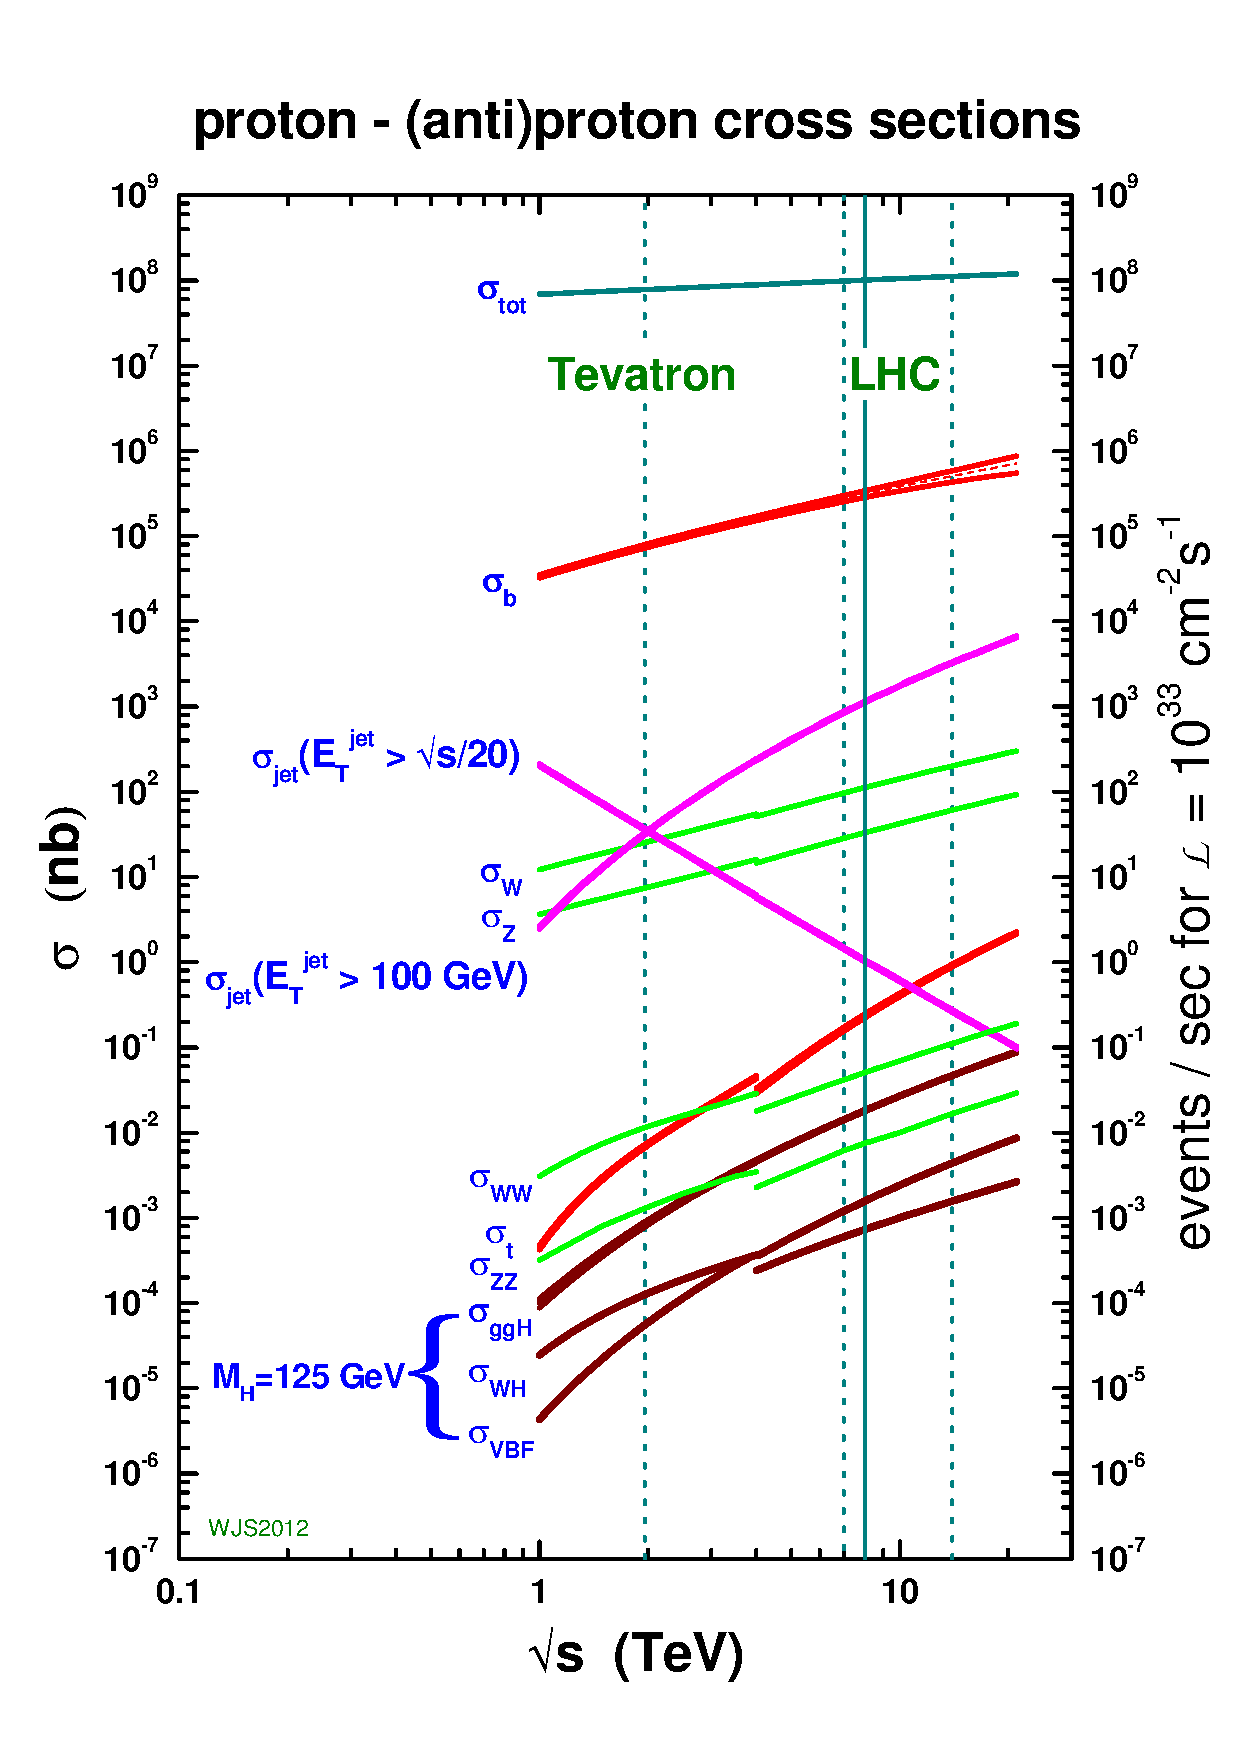
\includegraphics[width=0.40\textwidth,trim=0 2cm 0 0]{figures/crosssections2012_v5}
      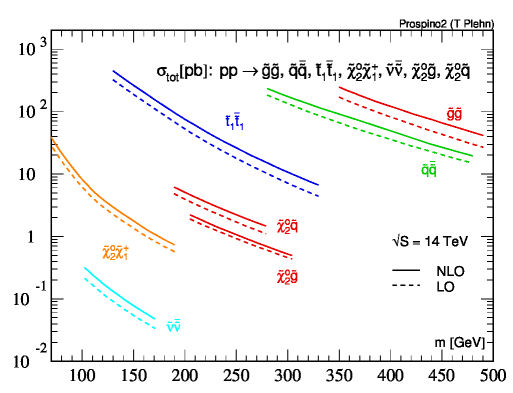
\includegraphics[width=0.40\textwidth,]{figures/PEacs.png}
      \caption{\label{fig:int_lumi} the lhc}
  \end{center}
\end{figure}

The potentially tiny rate of sparticle production compared with that
of known processes presents a challenge for the search. In addition, given the total
inelastic cross section of order 50 mb, the luminosity per colliding pair of bunches
achieved at the LHC is sufficiently high that the expected number of interactions that
occur in the same crossing as an interaction of interest is non-negligible. For the data
used in this search, the mean number of such “pile-up” interactions is approximately
13. Quarks or gluons which emerge from a hard-scattering process fragment and eventually 
group into hadrons before observation in a detector. They are visible as energetic
sprays of hadrons called “jets”, which typically leave tracks in the inner detector
and deposit energy in the calorimeters. The center-of-mass of the scattering system
has a boost along the beam-line which varies event-by-event. It is therefore convenient
to discuss jets (as well as other reconstructed particles) in terms of these quantities:
transverse momentum $\pt$ , which is invariant under such boosts, or similarly transverse
energy $\equiv E \sin\left(\theta\right)$, with $0 \leq \theta \leq \pi$ where $\theta$
is the polar angle from the beam-line; and pseudo-rapidity $\eta \equiv −\ln\left( \tan\left(\theta/2\right)\right)$
, of which differences are (approximately) invariant.


